\documentclass{article}

\usepackage[dvips]{graphicx}

\usepackage{natbib}
\bibliographystyle{apa}

\usepackage{url}

\newenvironment{eqnnon}{\begin{equation}}{\end{equation}}
\newenvironment{eqnarraynon}{\begin{eqnarray}}{\end{eqnarray}}

\newcommand{\mat}{A}
\newcommand{\sol}{b}
\newcommand{\eqmat}{F}
\newcommand{\eqvec}{h}
\newcommand{\ineqmat}{G}
\newcommand{\ineqvec}{k}

\newcommand{\cost}{c}
\newcommand{\eqfn}{f}
\newcommand{\ineqfn}{g}

\newcommand{\coord}{x}

\title{Solving constrained least squares problems}

\begin{document}

\tableofcontents

\section{Introduction}

We are interested in solving constrained least squares problems of 
the following form:
\begin{equation}
	\min_{\vec \coord} | \mat \vec \coord - \vec \sol |
	\label{least_squares}
\end{equation}
subject to both equality constraints:
\begin{equation}
	\eqmat \vec \coord = \vec \eqvec 
\end{equation}
and inequality constraints:
\begin{equation}
	\ineqmat \vec \coord \ge \vec \ineqvec
\end{equation}
Such problems are ubiquitous in machine learning applications.
Examples include the support vector machine dual problem, solving
for multi-class probabilities, and local approximations for iterative 
``global'' nonlinear optimizers.
This short summary discusses methods of tackling these types of problems.

\section{Lagrange multipliers}

Let $\cost$ be a (nonlinear) function to be minimized and let $\lbrace \eqfn_i \rbrace$ be a set of functions describing equality constraints:
\begin{equation}
	\eqfn_i(\vec \coord) = 0
 	\label{equality2}
\end{equation}
We can use a Lagrange multiplier to add the constraint to the optimization
problem:
\begin{equation}
	\min_{\lbrace \vec \coord, \vec \lambda \rbrace} \left \lbrace \cost(\vec \coord) + \sum_i \lambda_i \eqfn_i(\vec \coord) \right \rbrace
\end{equation}
where $\vec \lambda=\lbrace \lambda_I \rbrace$ are a set of {\it Lagrange multipliers}.
Taking the gradient and setting it to zero:
\begin{equation}
	\nabla_{\vec \coord} \cost + \sum_i \lambda_i \nabla_{\vec \coord} \eqfn_i = 0 
	\label{lagrange2}
\end{equation}
Note that taking the derivative with respect to the Lagrange multiplier
returns the equality constraint in (\ref{equality2}).
For the least squares problem in (\ref{least_squares}), 
Equation (\ref{lagrange2}) reduces to:
\begin{equation}
	\mat^T \mat \vec \coord + \vec \lambda \eqmat = \mat^T \vec \sol
\end{equation}
\citep{Lawson_Hanson1995}

\begin{figure}
	\includegraphics[width=0.9\textwidth]{Lagrange.eps}
	\caption{Illustration of Lagrange multiplier technique for equality constraints.}
\end{figure}


\section{Kuhn-Tucker conditions}

\bibliography{../ML_learning}

\end{document}


